\section*{Appendix}
\section{Wave Equation in 1+1 Dimensions with Periodic Boundary Conditions}

In section \ref{sec:simple_wave}, we refer that the code developed also provides results with a 4th order accuracy in space. The norm convergence of this results is found on figure \ref{fig:norm_simple_wave_4th_order} and the pointwise convergence is on figure \ref{fig:point_simple_wave_4th_order}.

\begin{figure}[H]
    \centering
    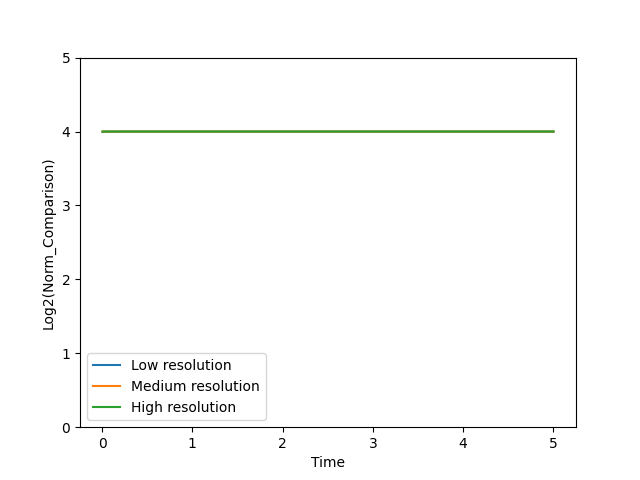
\includegraphics[width=0.9\columnwidth]{Images/simple_wave-4th-norm.png}
    \caption{Norm convergence of the solution to the wave equation in 1+1 dimensions with periodic boundary conditions and initial conditions represented in equation \ref{eq:sin_IC} in the 4th-order accurate in space and 1st-order accurate in time code}
    \label{fig:norm_simple_wave_4th_order}
\end{figure}

\begin{figure}[H]
    \centering
    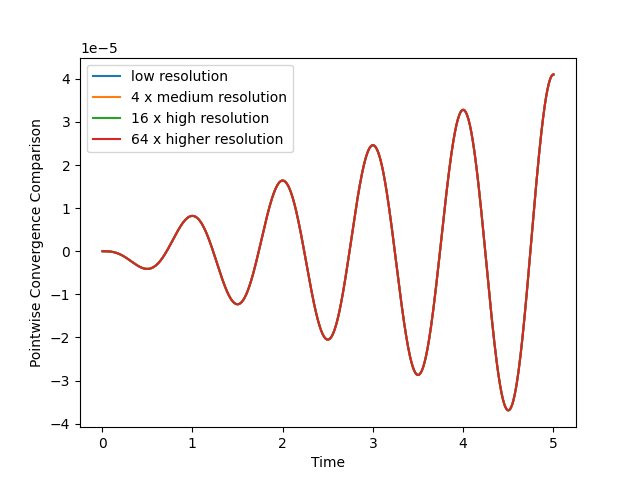
\includegraphics[width=0.9\columnwidth]{Images/simple_wave-4th-point.png}
    \caption{Pointwise convergence for $x = 0$ of the solution to the wave equation in 1+1 dimensions with periodic boundary conditions and initial conditions represented in equation \ref{eq:sin_IC} in the 4th-order accurate in space and 1st-order accurate in time code}
    \label{fig:point_simple_wave_4th_order}
\end{figure}

\newpage


\section{Non-linear Wave Equation in 1+1 Dimensions with Periodic Boundary Conditions}

In section \ref{sec:non_linear_wave}, we refer that the code developed also provides results with a 4th order accuracy in space. We can find the norm convergence for the results on figure \ref{fig:norm_non_linear_simple_wave_4th_order-diss} and the pointwise convergence is on figure \ref{fig:point_non_linear_simple_wave_4th_order-diss}.

\begin{figure}[H]
    \centering
    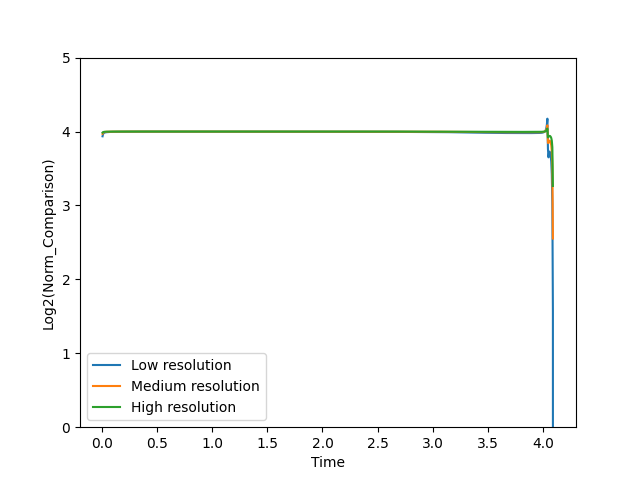
\includegraphics[width=0.9\columnwidth]{Images/non_linear_simple_wave-4th-norm-diss.png}
    \caption{Norm convergence of the solution to the non-linear wave equation in 1+1 dimensions (with artificial dissipation $\sigma = 0.007$) with periodic boundary conditions and initial conditions represented in equation \ref{eq:sin_IC} with $m = 2$ in the 4th-order accurate in space and 1st-order accurate in time code}
    \label{fig:norm_non_linear_simple_wave_4th_order-diss}
\end{figure}

\begin{figure}[H]
    \centering
    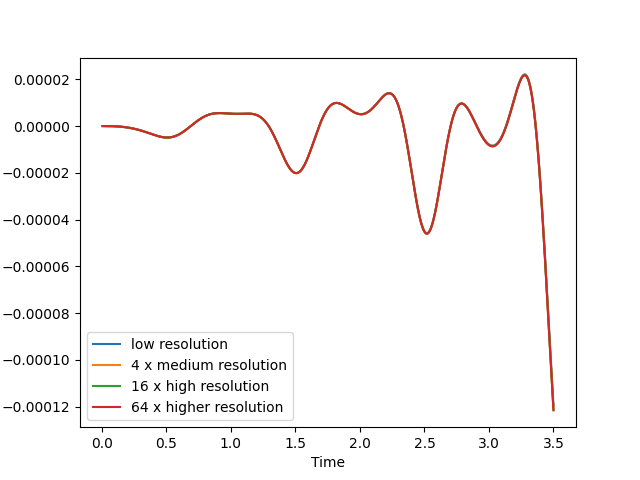
\includegraphics[width=0.9\columnwidth]{Images/non_linear_simple_wave-4th-point-diss.png}
    \caption{Pointwise convergence for $x = 0$ of the solution to the non-linear wave equation in 1+1 dimensions (with artificial dissipation $\sigma = 0.007$) with periodic boundary conditions and initial conditions represented in equation \ref{eq:sin_IC} with $m = 2$ in the 4th-order accurate in space and 1st-order accurate in time code}
    \label{fig:point_non_linear_simple_wave_4th_order-diss}
\end{figure}

\clearpage

\section{Linear Wave Equation in 3+1 Dimensions with Spherical Symmetry}

In section \ref{sec:spherical_wave}, we refer that the code developed also provides results with a 4th order accuracy in space. The norm convergence of this solution is found on figure \ref{fig:norm_spherical_wave_4th_order} and the pointwise convergence is on figure \ref{fig:point_spherical_wave_4th_order}.

\begin{figure}[H]
    \centering
    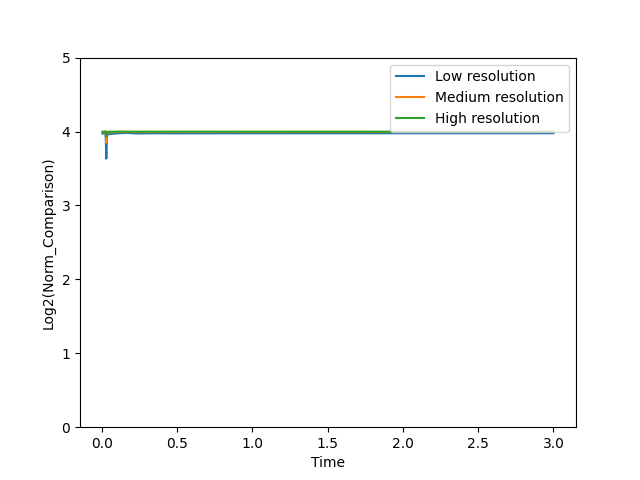
\includegraphics[width=0.9\columnwidth]{Images/spherical_wave-4th-norm.png}
    \caption{Norm convergence of the solution to the wave equation in 3+1 dimensions with spherical symmetry (with artificial dissipation $\sigma = 0.007$), imposing the parity of the solution at the origin and forcing the wave to 0 at "infinity", while providing initial conditions represented in equation \ref{eq:exp_IC} in the 4th-order accurate in space and 1st-order accurate in time code}
    \label{fig:norm_spherical_wave_4th_order}
\end{figure}

\begin{figure}[H]
    \centering
    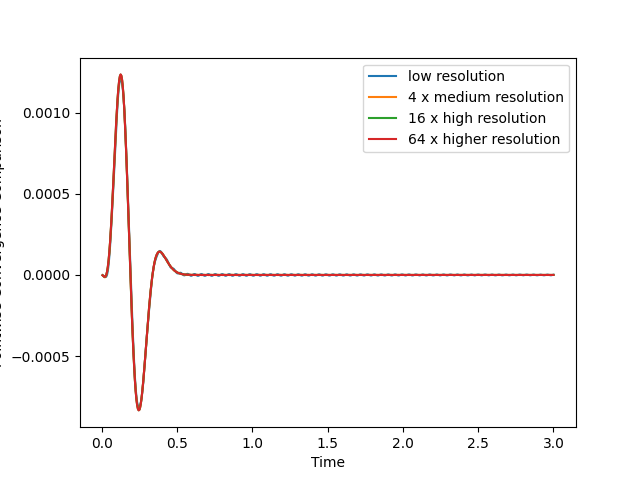
\includegraphics[width=0.9\columnwidth]{Images/spherical_wave-4th-point.png}
    \caption{Pointwise convergence for $x = 0$ of the solution to the wave equation in 3+1 dimensions with spherical symmetry (with artificial dissipation $\sigma = 0.007$), imposing the parity of the solution at the origin and forcing the wave to 0 at "infinity", while providing initial conditions represented in equation \ref{eq:exp_IC} in the 4th-order accurate in space and 1st-order accurate in time code}
    \label{fig:point_spherical_wave_4th_order}
\end{figure}

\newpage

\section{First-order Reduction of the ADM Evolution Equations in 3+1 Dimensions with Spherical Symmetry}

In section \ref{sec:adm}, we do not show the convergence tests for every field, as they are similar to one another. The plots for the norm convergence of $B$, $K_A$ and $K_B$ are shown in figures \ref{fig:norm_B}, \ref{fig:norm_KA} and \ref{fig:norm_KB} respectively, while the pointwise convergence of $B$ and $K_B$ are in figures \ref{fig:point_B} and \ref{fig:point_KB}. 

We also do not show the convergence plots for the auxiliary quantities $D_A$, $D_B$ and $\lambda$ in the main text. The norm convergence for these fields are shown in figures \ref{fig:norm_DA}, \ref{fig:norm_DB} and \ref{fig:norm_lambda}, while the pointwise convergence is found in figures \ref{fig:point_DA}, \ref{fig:point_DB} and \ref{fig:point_lambda}. 

Finally, we also refer the reduction constraints for $A$ and $B$, which is not shown in the main text. They are found in figures \ref{fig:red_A} and \ref{fig:red_B}

\begin{figure}[H]
    \centering
    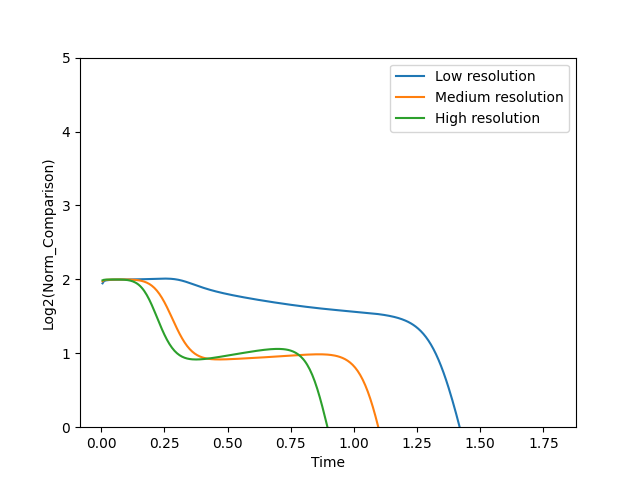
\includegraphics[width=0.9\columnwidth]{Images/B-norm.png}
    \caption{Norm convergence of the evolution of $B$ (with artificial dissipation $\sigma = 0.02$) while imposing the parity of the fields at the origin and not evolving "infinity", giving initial conditions represented in equation \ref{eq:GR_IC}}
    \label{fig:norm_B}
\end{figure}

\newpage

\begin{figure}[H]
    \centering
    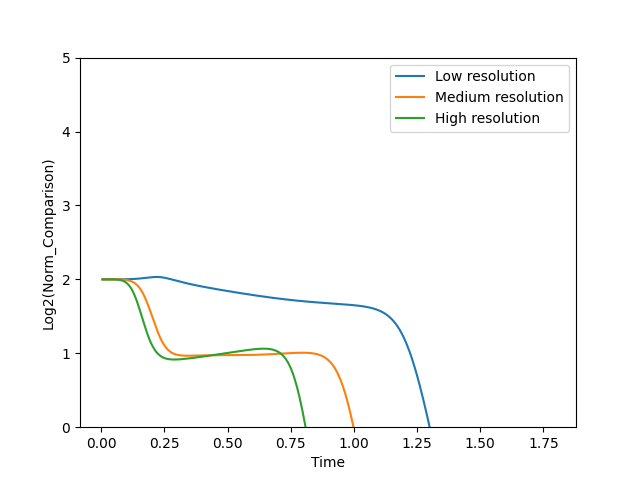
\includegraphics[width=0.9\columnwidth]{Images/KA-norm.png}
    \caption{Norm convergence of the evolution of $K_A$ (with artificial dissipation $\sigma = 0.02$) while imposing the parity of the fields at the origin and not evolving "infinity", giving initial conditions represented in equation \ref{eq:GR_IC}}
    \label{fig:norm_KA}
\end{figure}

\begin{figure}[H]
    \centering
    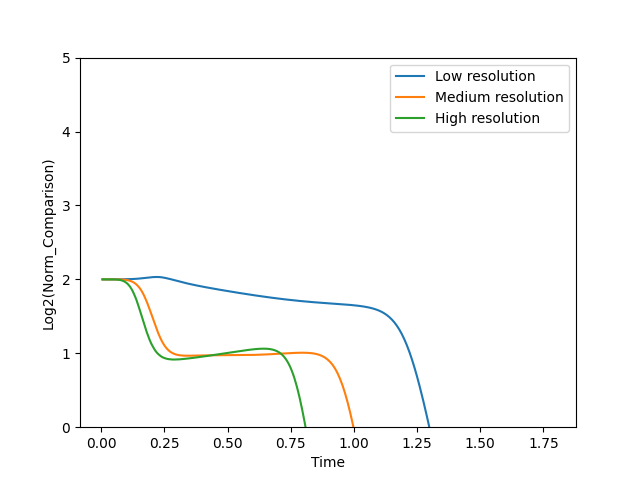
\includegraphics[width=0.9\columnwidth]{Images/KB-norm.png}
    \caption{Norm convergence of the evolution of $K_B$ (with artificial dissipation $\sigma = 0.02$) while imposing the parity of the fields at the origin and not evolving "infinity", giving initial conditions represented in equation \ref{eq:GR_IC}}
    \label{fig:norm_KB}
\end{figure}

\newpage

\begin{figure}[H]
    \centering
    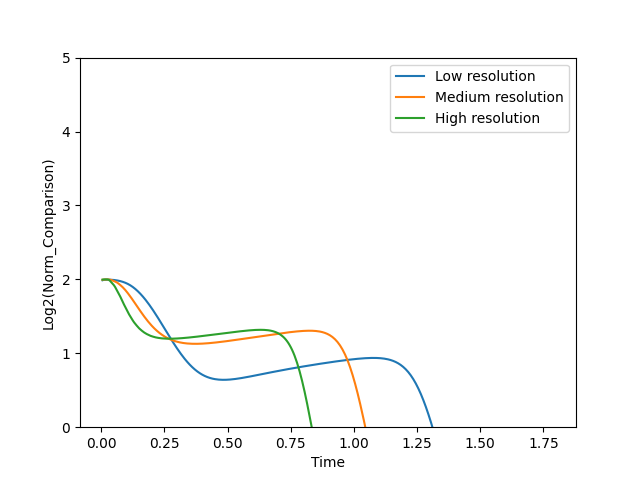
\includegraphics[width=0.9\columnwidth]{Images/DA-norm.png}
    \caption{Norm convergence of the evolution of $D_A$ (with artificial dissipation $\sigma = 0.02$) while imposing the parity of the fields at the origin and not evolving "infinity", giving initial conditions represented in equation \ref{eq:GR_IC}}
    \label{fig:norm_DA}
\end{figure}

\begin{figure}[H]
    \centering
    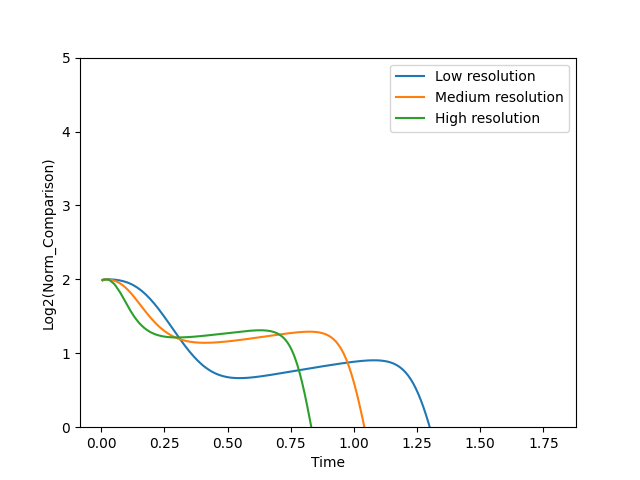
\includegraphics[width=0.9\columnwidth]{Images/DB-norm.png}
    \caption{Norm convergence of the evolution of $D_B$ (with artificial dissipation $\sigma = 0.02$) while imposing the parity of the fields at the origin and not evolving "infinity", giving initial conditions represented in equation \ref{eq:GR_IC}}
    \label{fig:norm_DB}
\end{figure}

\newpage

\begin{figure}[H]
    \centering
    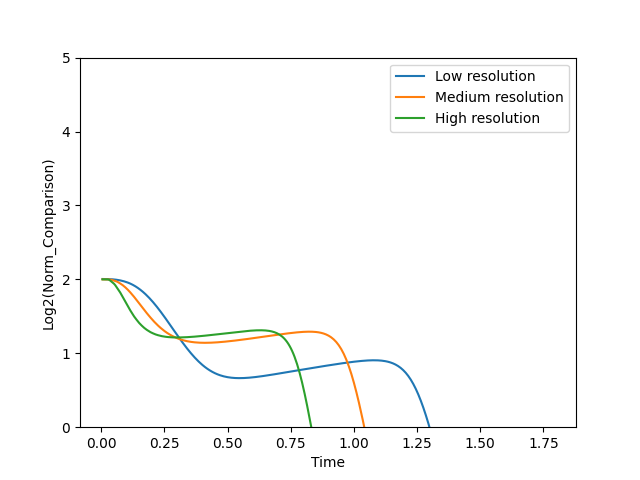
\includegraphics[width=0.9\columnwidth]{Images/lambda-norm.png}
    \caption{Norm convergence of the evolution of $\lambda$ (with artificial dissipation $\sigma = 0.02$) while imposing the parity of the fields at the origin and not evolving "infinity", giving initial conditions represented in equation \ref{eq:GR_IC}}
    \label{fig:norm_lambda}
\end{figure}

\begin{figure}[H]
    \centering
    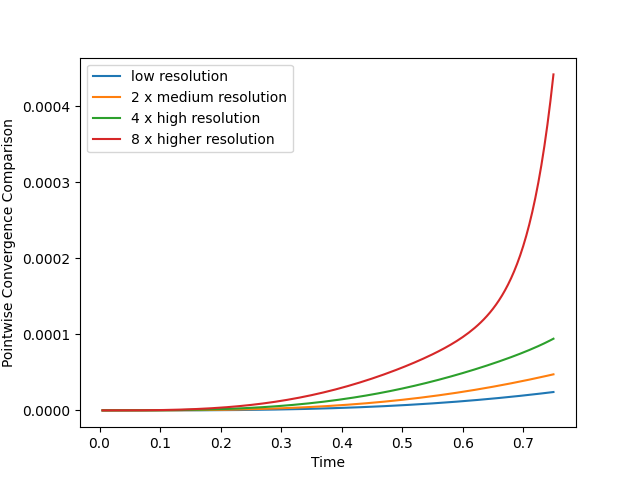
\includegraphics[width=0.9\columnwidth]{Images/B-point.png}
    \caption{Pointwise convergence at position $x = 0$ of the evolution of $B$ (with artificial dissipation $\sigma = 0.02$) while imposing the parity of the fields at the origin and not evolving "infinity", giving initial conditions represented in equation \ref{eq:GR_IC}}
    \label{fig:point_B}
\end{figure}

\newpage

\begin{figure}[H]
    \centering
    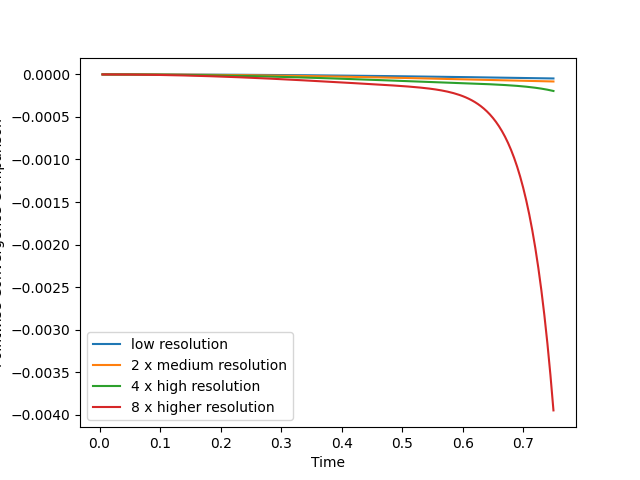
\includegraphics[width=0.9\columnwidth]{Images/KB-point.png}
    \caption{Pointwise convergence at position $x = 0$ of the evolution of $K_B$ (with artificial dissipation $\sigma = 0.02$) while imposing the parity of the fields at the origin and not evolving "infinity", giving initial conditions represented in equation \ref{eq:GR_IC}}
    \label{fig:point_KB}
\end{figure}

\begin{figure}[H]
    \centering
    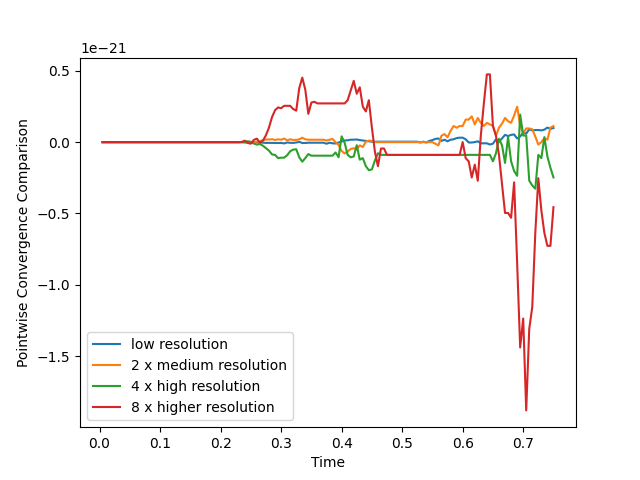
\includegraphics[width=0.9\columnwidth]{Images/DA-point.png}
    \caption{Pointwise convergence at position $x = 0$ of the evolution of $D_A$ (with artificial dissipation $\sigma = 0.02$) while imposing the parity of the fields at the origin and not evolving "infinity", giving initial conditions represented in equation \ref{eq:GR_IC}}
    \label{fig:point_DA}
\end{figure}

\newpage

\begin{figure}[H]
    \centering
    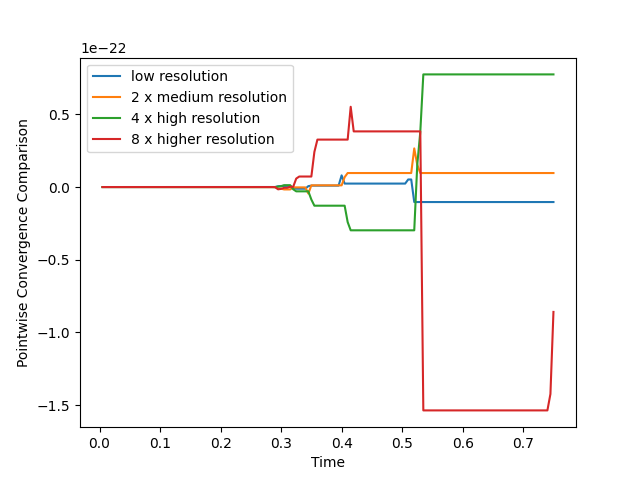
\includegraphics[width=0.9\columnwidth]{Images/DB-point.png}
    \caption{Pointwise convergence at position $x = 0$ of the evolution of $D_B$ (with artificial dissipation $\sigma = 0.02$) while imposing the parity of the fields at the origin and not evolving "infinity", giving initial conditions represented in equation \ref{eq:GR_IC}}
    \label{fig:point_DB}
\end{figure}

\begin{figure}[H]
    \centering
    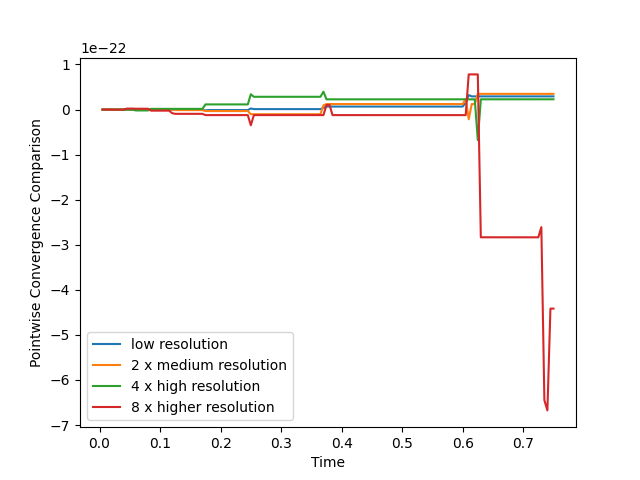
\includegraphics[width=0.9\columnwidth]{Images/lambda-point.png}
    \caption{Pointwise convergence at position $x = 0$ of the evolution of $\lambda$ (with artificial dissipation $\sigma = 0.02$) while imposing the parity of the fields at the origin and not evolving "infinity", giving initial conditions represented in equation \ref{eq:GR_IC}}
    \label{fig:point_lambda}
\end{figure}

\newpage

\begin{figure}[H]
    \centering
    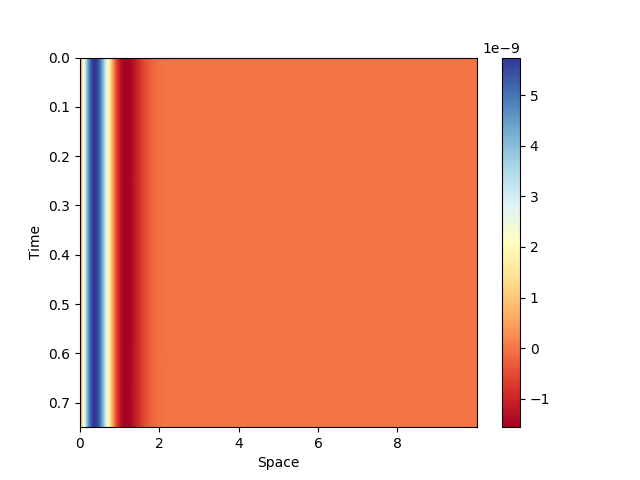
\includegraphics[width=0.9\columnwidth]{Images/adm_evolution-2nd_order-Reduction_A.png}
    \caption{Intensity plot of the reduction constraint for $A$ and $D_A$ constraint of the evolution, where we imposed the parity of the fields at the origin and have not evolved "infinity", giving initial conditions represented in equation \ref{eq:GR_IC}}
    \label{fig:red_A}
\end{figure}

\begin{figure}[H]
    \centering
    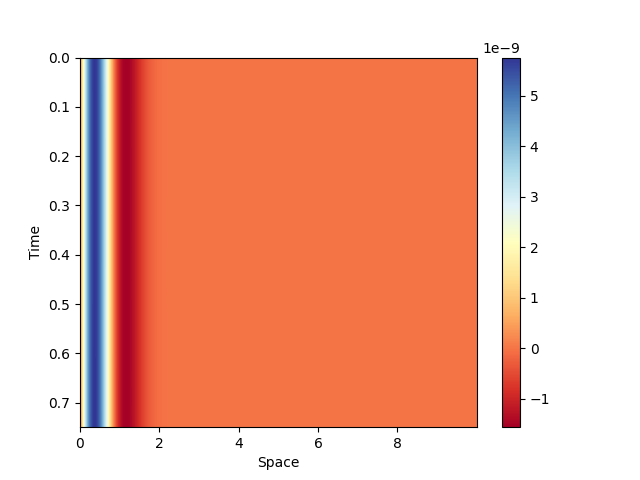
\includegraphics[width=0.9\columnwidth]{Images/adm_evolution-2nd_order-Reduction_B.png}
    \caption{Intensity plot of the reduction constraint for $B$ and $D_B$ constraint of the evolution, where we imposed the parity of the fields at the origin and have not evolved "infinity", giving initial conditions represented in equation \ref{eq:GR_IC}}
    \label{fig:red_B}
\end{figure}

\newpage